%Chap 3 pag 54
\definecolor{DarkRed}{RGB}{128,0,0}
\definecolor{Green}{RGB}{0,100,0}
\begin{frame}{Búsqueda en profundidad}
Expandir el nodo no expandido más profundo.\\
\textcolor{DarkRed}{Implementación:}
\begin{center}
    \textit{\textcolor{Green}{franja}} = cola LIFO, es decir, poner sucesores al
    frente.\\
\end{center}
\begin{figure}
    \centering
    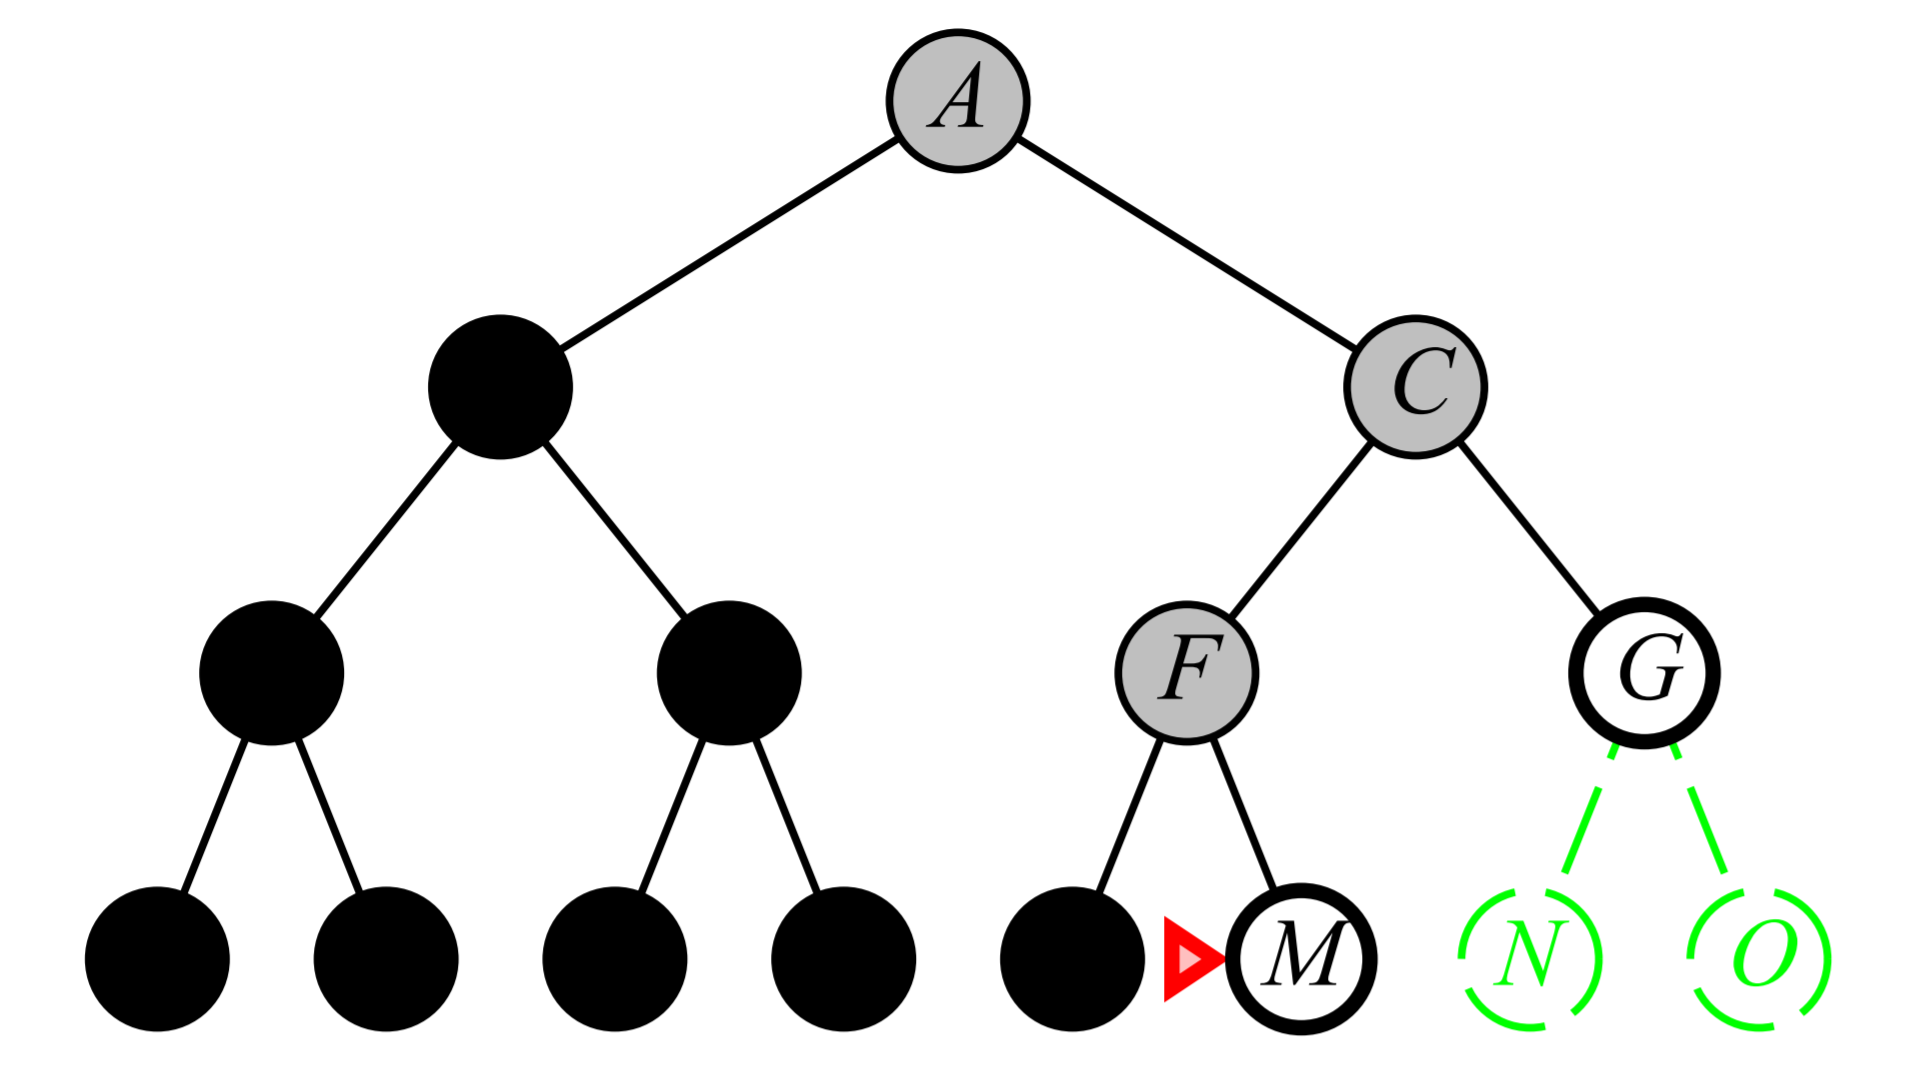
\includegraphics[width = 60mm, scale = 0.7]{images/54_image.PNG}
\end{figure}
\end{frame}{}
